\documentclass[12pt,UTF8]{ctexart}
\usepackage{titling,setspace}
\usepackage{enumerate,enumitem}
\usepackage{amsmath,amssymb,amsfonts}
\usepackage{listings}
\usepackage{comment}
\usepackage{float}
\usepackage{graphicx}
\usepackage{multicol,multirow}
\usepackage[unicode=true,%本行非常重要 支持中文目录hyperref CJKbookmarks对二级目录没用
	colorlinks,
	linkcolor=black,
	anchorcolor=black,
	citecolor=black,
	CJKbookmarks=false]{hyperref}
\usepackage{xcolor}
\usepackage{geometry}
\geometry{top=25mm,bottom=25mm,left=25mm,right=25mm}
\pagestyle{plain}%删除页眉
\CTEXsetup[format={\large\bfseries}]{section}
\renewcommand\maketitlehooka{\null\mbox{}\vfill} % 标题页
\renewcommand\maketitlehookd{\vfill\null}

\lstset{language=c++,basicstyle=\tiny,escapechar=`,showstringspaces=false}
\setlength{\droptitle}{-100pt}%减少标题与页眉距离

\setenumerate[1]{itemsep=0pt,partopsep=0pt,parsep=\parskip,topsep=5pt}
\setitemize[1]{itemsep=0pt,partopsep=0pt,parsep=\parskip,topsep=5pt}

\title{{\Huge Project 2\\机场模拟}}

\vspace{100pt}
\author{\vspace{200pt}\quad\\
计科一班 17341009 曾天宇\\
计科一班 17341015 陈鸿峥\\
计科二班 17341059 黄杨峻}
\date{}

\begin{document}
\begin{spacing}{1.4}

\clearpage\maketitle
\thispagestyle{empty}

\newpage
\setcounter{page}{1}
\section{题目要求}
	书本在P96-P109中提供了一个机场模拟器的实现代码。首先我们分别有两个队列,一个控制起飞一个控制降落,而我们拥有一个供飞机起飞降落的跑道(每次只能进行起飞或者降落中的一个操作)。飞机的起降数目由随机函数生成,每个时刻进入起飞序列或降落序列的飞机数目都满足泊松分布。程序输入为起降队列的长度限制,机场运作的总时间、起飞飞机的比率、降落飞机的比率,程序的输出为机场各跑道起降情况、飞机入队情况以及模拟结束后各种数据的汇总。

	这次的项目将在上述机场模拟器的基础上,分别实现以下六个要求:
	
	\begin{itemize}
		\item 整合书中的程序,并做几组实验,调整起降飞机的数目,找出尽可能大的合适参数使得飞机尽可能不被机场拒绝起降,并探究队列大小的改变会对结果造成怎样的影响。
		\item 把机场跑道数改为两条,一条只用于降落另一条只用于起飞,比较跑道数倍增后机场的客机吞吐量是否多于原来的两倍。
		\item 机场跑道数仍为两条,一条主要用于降落另一条主要用于起飞。当其中一条跑道闲置的时候,可为另一条跑道分流;当着陆队列满后,两条跑道都将被用于着陆,直到着陆序列为空。
		\item 跑道数目增加到三条,第三条跑道主要用于飞机降落,当着陆队列为空时可用于起飞。
		\item 回到单跑道状态,为飞机添加一个燃油量属性,燃料以剩余时间作为单位。若飞机燃料不足,则其可被允许优先降落。探究在此情况下,机场的最大吞吐量。
		\item 去除随机函数,通过用户输入指定每一个时间单位的起降飞机数目,以便调试。
	\end{itemize}
	
\section{数据结构与算法}
	这题考察的数据结构是\textbf{队列},是一个\textbf{先进先出}的结构。本题涉及到两个队列---起飞队列和着陆队列,我们用\verb'push()'和\verb'pop()'函数来控制入队和出队。由于六个小题涉及到的类相同,仅仅是成员函数的不同,因此我们将所有代码都集成到了一个程序中,通过命令行直接传入参数(问题的编号)来控制程序功能,这是我们程序的一个亮点所在。
	
	\textbf{题一}较为简单,先将课本中的代码部分(包括Appendix中的随机数)进行代码整合,然后通过输入不同的arrival\_rate和departure\_rate组合进行测试。实验结果在章节\ref{sec:exp}给出。
	
	\textbf{题二}则类似题一,只是增加了一条跑道。由于跑道的职能类似,实现较简单,唯一不同就是要在输出部分确定飞机从哪个跑道起飞或降落。在这里我们使用一个\verb'vector'容器来储存不同的runway,而对于某一条runway,其可以四种状态中的某一种,包括:主要用于着陆(mainly\_landing)、主要用于起飞(mainly\_takeoff)、仅用于着陆(only\_landing)、仅用于起飞(only\_takeoff)。初始两条跑道状态为only\_landing和only\_takeoff,然后分别掌管各自队列的任务即可。注意,这里我们发现了各个问题之间的共同之处,并将问题的结构进行抽象,最终抽象出四种跑道的状态,这也是我们程序的一大亮点。
	
	\textbf{题三}在题二的基础上稍有改动,两条跑道的初始状态改为mainly\_landing和mainly\_takeoff,当降落或起飞的某一条队列为空时,对应跑道即可进行另外一种操作。如降落队列为空,mainly\_landing跑道便可执行起飞操作。此外,本题还增加了剩余队列清理(backlog clear)功能,当降落队列满时两个跑道同时用于清空降落队列,直到降落队列为空,输出``Landing backlog cleared''提示。注意本题我们用了一个类似有限状态机的写法,在\verb'Runway'类内构造了一个change\_runway\_status成员函数,用于更改跑道的不同状态。
	
	\textbf{题四}在题二的基础上增加了一条状态为mainly\_landing的跑道,实现方法与题三基本相同,在此不再赘述。
	
	\textbf{题五}要求我们对飞机添加油量这一参数,并设定一定的算法使得飞机尽可能不要因为燃油不足而坠毁。对于这个问题,我们优先对燃油量较低的飞机进行降落。如果燃油不足以使得飞机飞到机场,则飞机进入紧急状态,并暂停机场中一切起飞和降落活动,对紧急状态飞机进行优先降落。为增强整个算法的正确性和健壮性,我们对航油不足的情况进行相应的分析,并查阅了《民用航空空中交通管理规则 (CCAR-93-R5)》中的相关规定:
	\begin{itemize}
		\item 第四百八十四条\qquad最低油量表示航空器燃油油量已达到不能再耽搁的状态。最低油量非指紧急状况,仅表示如果再出现不适 当耽搁很可能发生紧急状况。当航空器报告最低油量时,管制员应当:
		\begin{itemize}
			\item 尽可能保障航空器按照计划航迹飞行,减少不必要的飞行延迟和等待,防止航空器进入``紧急油量''状态;
			\item 及时将该航空器``最低油量''状况通报给将要移交的下一管制单位。
		\end{itemize}
	\end{itemize}

	因此,我们可以提前引导油量不足的飞机先行降落以减少伤亡。鉴于本题是一个单跑道情形,我们可以检测在每一架飞机的油量,如果遇到即将遇险的飞机,可以安排其与前机在同一个时间段内降落。具体到程序,我们给每一架飞机增加了一个fuel成员,并添加一个reduce\_fuel函数,当某架飞机的燃油量小于一个阈值时,机场进入紧急状态。
	
	\textbf{题六}需要将随机函数更改为手工输入。故我们在程序中引入布尔参数\verb'manual_mode'(默认为假),通过命令行读入,若其为真时,随机函数变更为手动输入。注意我们这种实现方式是同时针对前面五个问题都可以使用的,大大增强了代码的可用性。

	最后值得一提的是,我们的程序对原来课本的程序进行进一步的抽象、优化、代码整合,使得代码结构更加清晰易懂。如将\verb'main'函数中关于moving\_plane的部分整合入activity中,保证类关系的一致性,同时去除无意义的参数传递。

\section{测试数据、结果及分析}
\label{sec:exp}
% (所输入的数据及相应的运行结果,运行结果要有提示信息,运行结果采用截图方式给出。)
我们对每一个问题都做了多组实验,这里对于每个问题都仅展示两组实验结果,一组飞机量较为小,每个单位时间的飞机量小于1,另一组则飞机量较大,每个单位时间的飞机量大于1。通过这些实验,观察结果,得出结论。

\begin{figure}[H]
	\centering
	\begin{tabular}{cc}
	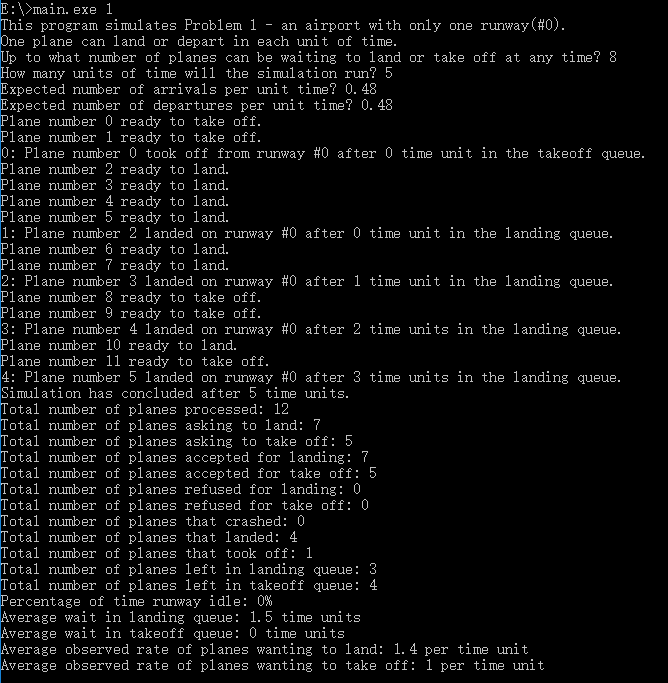
\includegraphics[width=0.5\linewidth]{fig/exp_10.PNG} &
	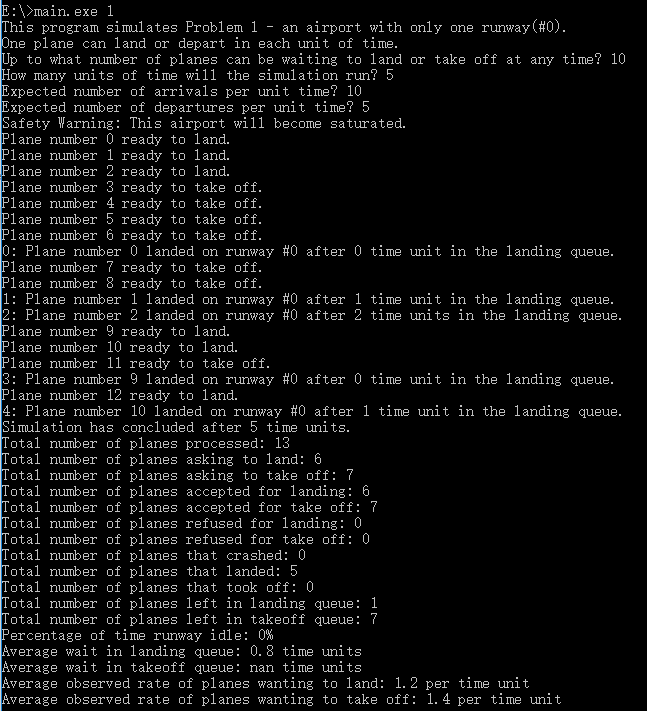
\includegraphics[width=0.5\linewidth]{fig/exp_11.PNG}
	\end{tabular}
	\caption{问题一实验结果}
	\label{fig:1}
\end{figure}
由图\ref{fig:1}可知:假设队列大小不变,模拟时间一定,当预期起飞和降落的数量之和最大且为队列大小的两倍时,飞机不太可能会被拒绝起飞和降落。如果其和超过两倍,被拒绝起飞或降落的可能性很大;因此两个数量的最优期望值是队列最大的情况,此时的机场运作效率最高。而通过改变输入的$\text{queue limit}$,我们得出的结论是:如果队列的最大值增大,而其它值不变,接受飞机起飞和降落的数量不变;如果队列最大值减少,其它值不变,接收的数量也会减少。

\begin{figure}[H]
	\centering
	\begin{tabular}{cc}
	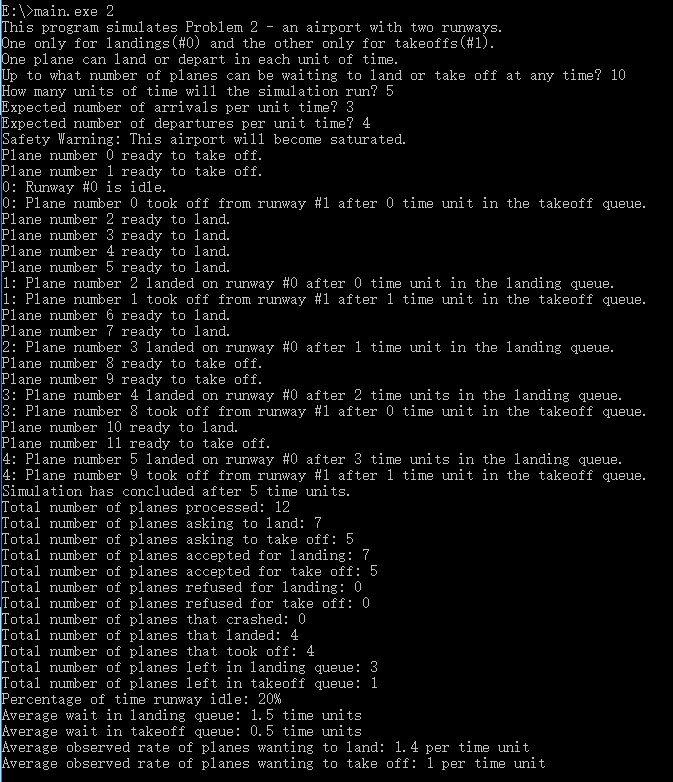
\includegraphics[width=0.5\linewidth]{fig/exp_20.PNG} &
	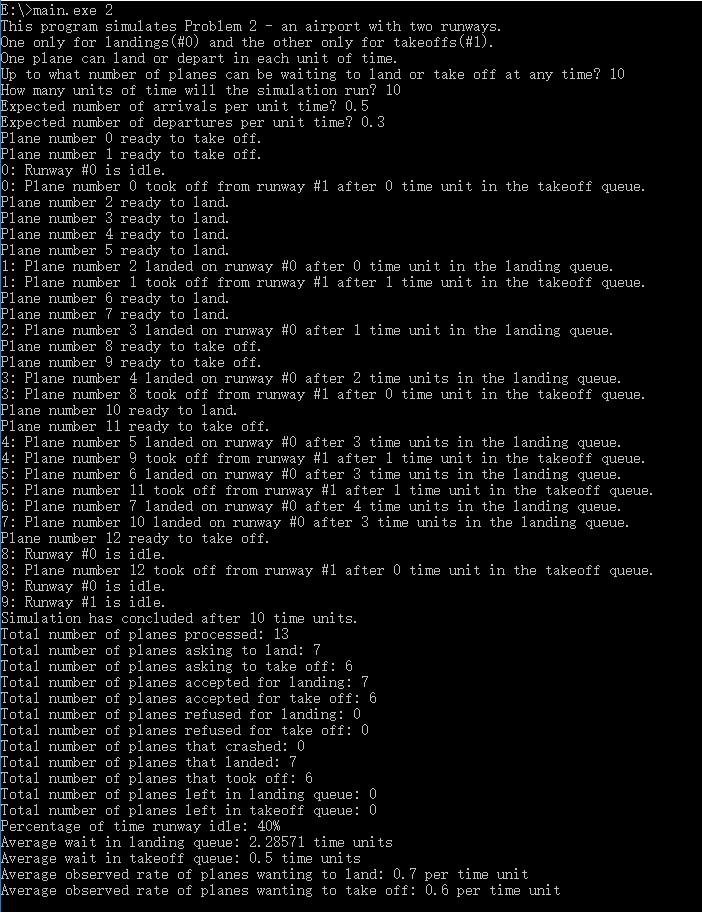
\includegraphics[width=0.5\linewidth]{fig/exp_21.PNG}
	\end{tabular}
	\caption{问题二实验结果}
	\label{fig:2}
\end{figure}
由图\ref{fig:2}可知:当飞机量较少,即机场远未及饱和状态时,添加跑道对最终飞机接收数目的影响并不大;而当飞机量过大,机场已经达到饱和状态时,添加一条跑道可以近乎实现成倍飞机接收量的增长。

\begin{figure}[H]
	\centering
	\begin{tabular}{cc}
	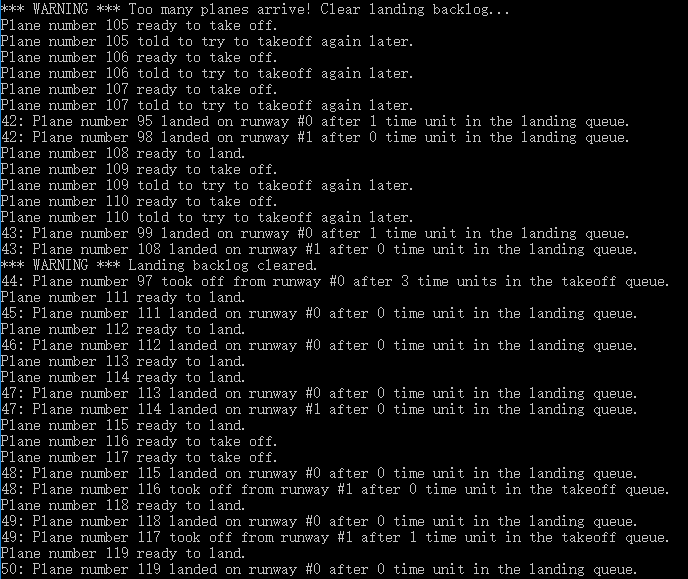
\includegraphics[width=0.5\linewidth]{fig/exp_30.PNG} &
	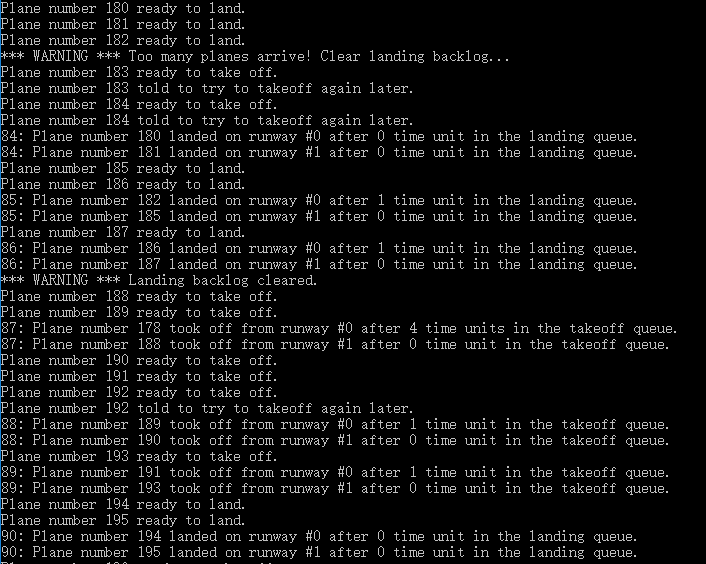
\includegraphics[width=0.5\linewidth]{fig/exp_31.PNG}
	\end{tabular}
	\caption{问题三实验结果}
	\label{fig:3}
\end{figure}
由图\ref{fig:3}可知:增加一条跑道而不特别指定跑道的作用,可以起到更好的效果,使吞吐率进一步提升。
图\ref{fig:3}中显示了WARNING状态,表明开始进行降落队列的清空。

\begin{figure}[H]
	\centering
	\begin{tabular}{cc}
	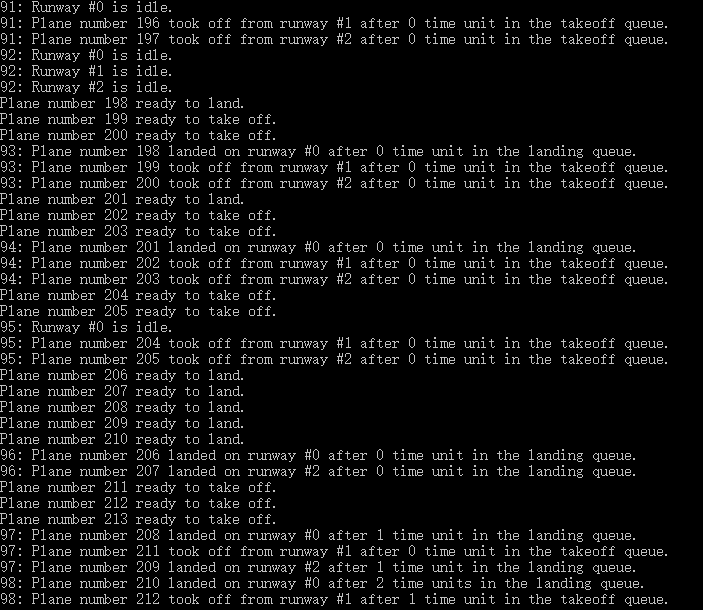
\includegraphics[width=0.5\linewidth]{fig/exp_40.PNG} &
	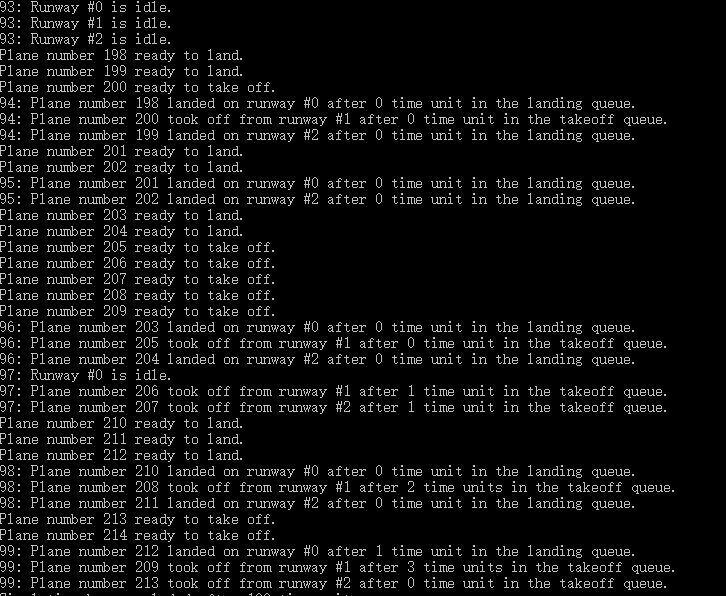
\includegraphics[width=0.5\linewidth]{fig/exp_41.PNG}
	\end{tabular}
	\caption{问题四实验结果}
	\label{fig:4}
\end{figure}
由图\ref{fig:4}可知:与问题二的结论类似,需要讨论机场是否达到饱和状态。饱和则新增跑道可增大吞吐量,否则则不行。但考虑到小机场较少飞机的情况,继续增加跑道只会增加成本,使得新增的跑道大多时候处在空闲的状态。

\begin{figure}[H]
	\centering
	\begin{tabular}{cc}
	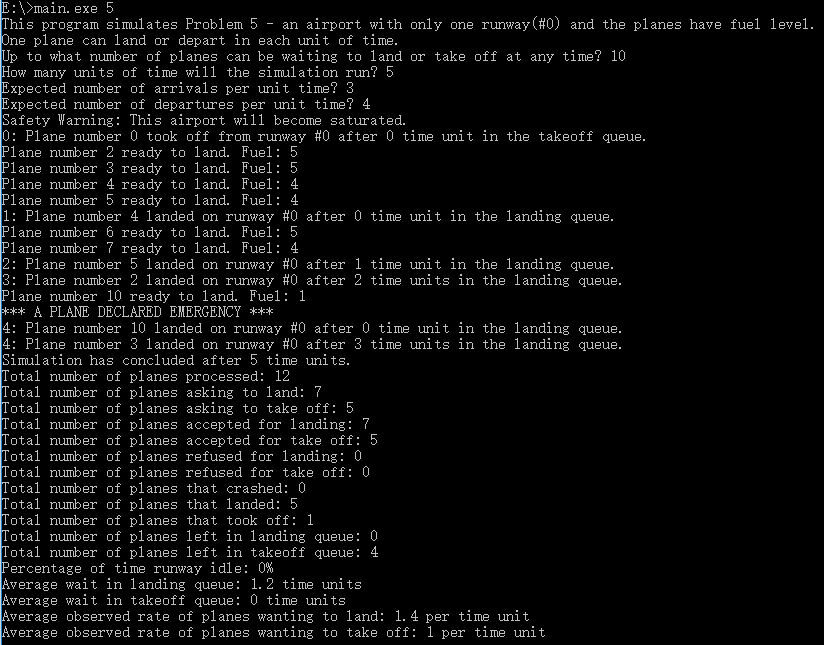
\includegraphics[width=0.5\linewidth]{fig/exp_50.PNG} &
	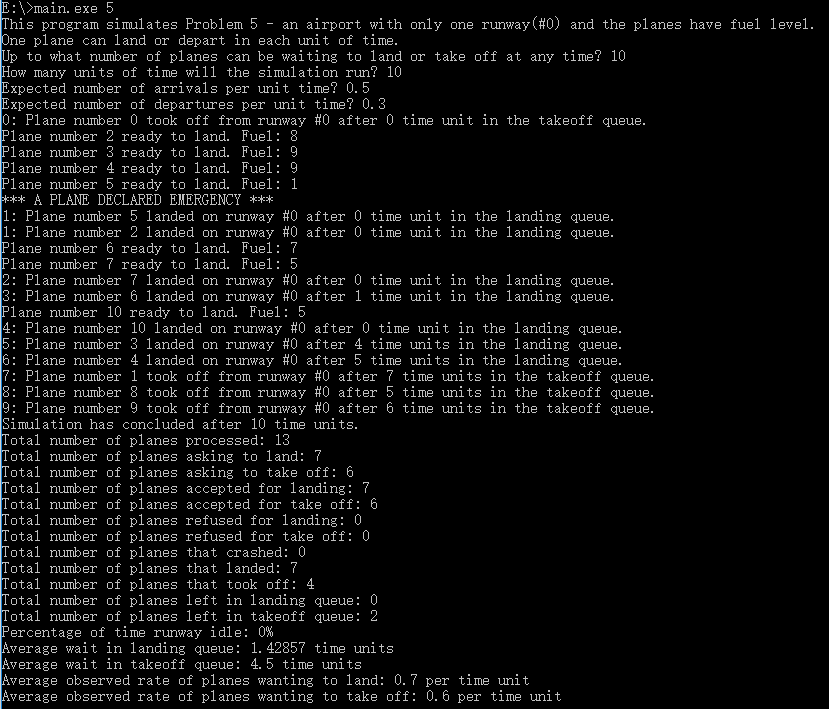
\includegraphics[width=0.5\linewidth]{fig/exp_51.PNG}
	\end{tabular}
	\caption{问题五实验结果}
	\label{fig:5}
\end{figure}
由图\ref{fig:5}可知:增加燃油限制,对吞吐量不会有太大影响,仅仅是将普通的队列更改为优先队列而已,先处理优先级较大(燃油量较少)的飞机。同时需要处理好紧急情况(EMERGENCY),在图\ref{fig:5}中出现了这种情况并被我们成功处理,可见我们的程序具有很强的鲁棒性。

\begin{figure}[H]
	\centering
	\begin{tabular}{cc}
	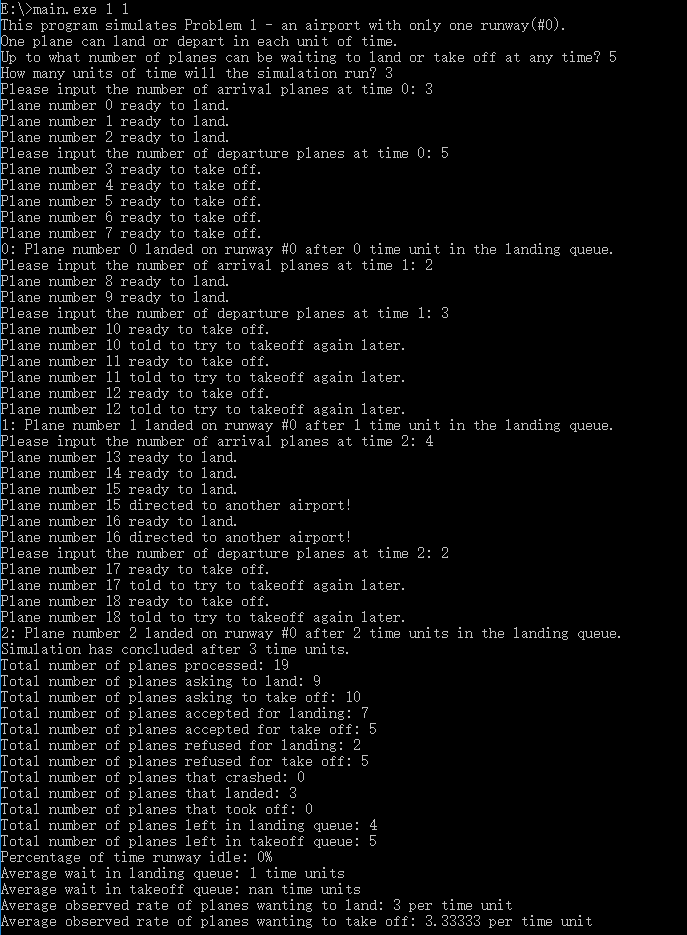
\includegraphics[width=0.5\linewidth]{fig/exp_60.PNG} &
	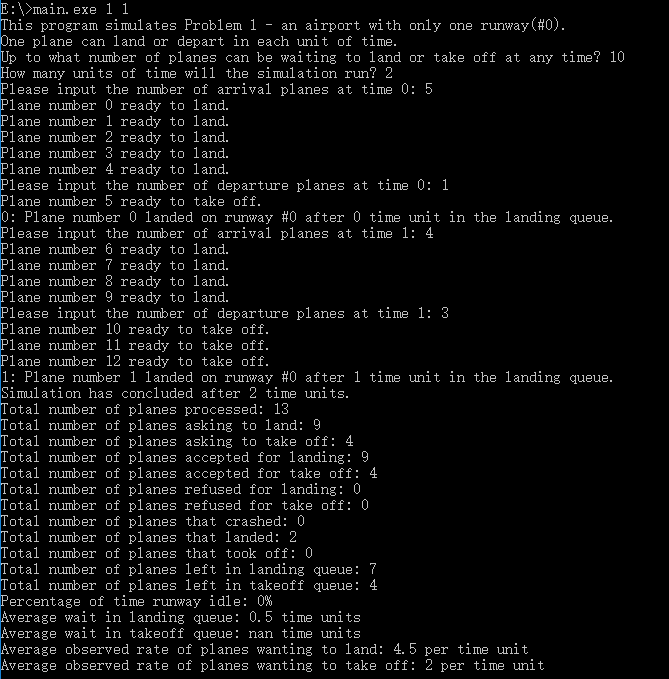
\includegraphics[width=0.5\linewidth]{fig/exp_61.PNG}
	\end{tabular}
	\caption{问题六实验结果}
	\label{fig:6}
\end{figure}
由图\ref{fig:6}可知:增加人工输入环节其实会使过程变得更加复杂,每个时刻到达与离去的飞机数目不再符合数学规律,但我们的程序依然能够很好地处理。


\section{分工、贡献与自我评分}
\begin{table}[H]
	\centering
	\begin{tabular}{|c|c|c|c|}
		\hline
		& 分工 & 贡献度 & 自我评分\\
		\hline
		曾天宇 & 复现书本代码,实现问题一、五,查阅资料,实验报告撰写 & 0.33 & 10/10\\
		陈鸿峥 & 复现书本代码,实现问题二、六,代码整合与测试,修改实验报告 & 0.33 & 10/10\\
		黄杨峻 & 复现书本代码,实现问题三、四,完成实验报告大部分内容 & 0.33 & 10/10\\
		\hline
	\end{tabular}
\end{table}

\section{项目总结}
% (收获、体会,若实验课上未完成调试,要认真找出错误并分析原因等。)
	虽然这次项目只是考察基本数据结构队列的使用以及相应的模拟,但如果要作为一个大项目来做也绝非易事。首先书本中的源代码就非常的长,非常的复杂,一开始需要花费不少时间读懂程序如何运作,而且要非常熟悉每一个函数及代码段的功能,脑力耗费自然也不小。一开始,我们小组还没定好代码编写的风格,最后才决定重构代码并将功能整合,所以前后浪费了不少时间。而且由于是小组作业,组内成员对题目的理解也各有不同,所以对于同一问题,各自的解决思路和代码也不同。到最后整合成一个程序时遇到了不少困难,可能下次做项目的时候要先统一好意见再开始。最好创建一个文档,并新建一个git仓库,共同管理,同时做好代码注释以便组员阅读。
\end{spacing}

\section{程序清单}
\subsection{主函数}
\begin{lstlisting}
#include <iostream>
#include <queue>
#include <vector>
#include <cstring>
#include <algorithm>
#include <time.h>
#include <cmath>
#include "Random.hpp"
#include "Runway.hpp"
using namespace std;

int problem_num;
bool manual_mode = false;

void initialize(int& end_time,int& queue_limit,double& arrival_rate,double& departure_rate)
{
    switch (problem_num)
    {
        case 1:
        cout << "This program simulates Problem 1 - an airport with only one runway(#0)." << endl;
        break;
        case 2:
        cout << "This program simulates Problem 2 - an airport with two runways." << endl
             << "One only for landings(#0) and the other only for takeoffs(#1)." << endl;
        break;
        case 3:
        cout << "This program simulates Problem 3 - an airport with two runways." << endl
             << "One mainly for landings(#0) and the other mainly for takeoffs(#1)." << endl;
        break;
        case 4:
        cout << "This program simulates Problem 4 - an airport with three runways." << endl
             << "One only for landings(#0), the second one only for takeoffs(#1), and the third mainly for landings(#2)." << endl;
        break;
        case 5:
        cout << "This program simulates Problem 5 - an airport with only one runway(#0) and the planes have fuel level." << endl;
        break;
        default:
        cerr << "Error: No such problem!" << endl;
        return;
    }
    cout << "One plane can land or depart in each unit of time." << endl;
    cout << "Up to what number of planes can be waiting to land or take off at any time? " << flush;
    cin  >> queue_limit;
    cout << "How many units of time will the simulation run? " << flush;
    cin  >> end_time;
    if (manual_mode)
        return;
    bool acceptable = false;
    do {
        cout << "Expected number of arrivals per unit time? " << flush;
        cin >> arrival_rate;
        cout << "Expected number of departures per unit time? " << flush;
        cin >> departure_rate;
        if (arrival_rate < 0.0 || departure_rate < 0.0)
            cerr << "These rates must be nonnegative." << endl;
        else
            acceptable = true;
        if (acceptable && arrival_rate + departure_rate > 1.0)
            cerr << "Safety Warning: This airport will become saturated." << endl;
    } while (!acceptable);
}

int main(int argc, const char * argv[]) {
    problem_num = stoi(string(argv[1]));
    if (argc > 2) // the second argv is for Problem 6 (used for debug)
        manual_mode = (stoi(string(argv[2])) == 1 ? 1 : 0);
    int end_time, queue_limit, flight_number=0;
    double arrival_rate, departure_rate;
    initialize(end_time, queue_limit, arrival_rate, departure_rate); // initialize the arrive and depart list
    Random variable; // set the number of planes to takeoff and land

    // initialize the airport and runways
    Runway small_airport(queue_limit);
    if (problem_num == 1 || problem_num == 5)
        small_airport.set_runways(1,
            vector<Runway_mode> {Runway_mode::mainly_landing});
    else if (problem_num == 2)
        small_airport.set_runways(2,
            vector<Runway_mode> {Runway_mode::only_landing,
                                 Runway_mode::only_takeoff});
    else if (problem_num == 3)
        small_airport.set_runways(2,
            vector<Runway_mode> {Runway_mode::mainly_landing,
                                 Runway_mode::mainly_takeoff});
    else if (problem_num == 4)
        small_airport.set_runways(3,
            vector<Runway_mode> {Runway_mode::only_landing,
                                 Runway_mode::only_takeoff,
                                 Runway_mode::mainly_landing});

    // processing
    bool flag_change_status = false;
    for (int current_time = 0; current_time < end_time; current_time++) {
        // generate arrival and departure planes
        int num_arrivals;
        if (!manual_mode)
            num_arrivals = variable.poisson(arrival_rate);
        else
        {
            cout << "Please input the number of arrival planes at time " << current_time << ": ";
            cin >> num_arrivals;
        }

        if (problem_num != 5)
            for (int i = 0; i < num_arrivals; i++) {
                Plane current_plane(flight_number++, current_time, Status::arriving);
                if (small_airport.can_land(current_plane) != true) {
                    current_plane.refuse();
                }
            }
        else {
            vector<Plane> arrival_plane;
            for (int i = 0; i < num_arrivals; i++) {
                Plane current_plane(flight_number++, current_time, Status::arriving, end_time); // end_time-current_time
                arrival_plane.push_back(current_plane);
            }
            // sort by planes' fuel
            sort(arrival_plane.begin(),arrival_plane.end(),[](const Plane& plane1, const Plane& plane2)
                {return plane1.get_fuel() < plane2.get_fuel();});
            for (int i = 0; i < num_arrivals; i++) {
                if (small_airport.can_land(arrival_plane[i], (problem_num == 5 ? 1 : 0)) != true) {
                    arrival_plane[i].refuse();
                }
            }
        }
        // clear landing backlog
        if (problem_num == 3 && small_airport.landing_full() && !flag_change_status)
        {
            cout << "*** WARNING *** Too many planes arrive! Clear landing backlog..." << endl;
            small_airport.change_runway_status(0,Runway_mode::only_landing);
            small_airport.change_runway_status(1,Runway_mode::only_landing);
            flag_change_status = true;
        }

        int num_departures;
        if (!manual_mode)
            num_departures = variable.poisson(departure_rate);
        else
        {
            cout << "Please input the number of departure planes at time " << current_time << ": ";
            cin >> num_departures;
        }
        for (int j = 0; j < num_departures; j++) {
            Plane current_plane(flight_number++, current_time, Status::departing);
            if (small_airport.can_depart(current_plane) != true) {
                current_plane.refuse();
            }
        }

        // process the planes in the queue
        small_airport.activity(current_time, (problem_num == 5 ? 1 : 0));

        // Problem 3 - clear the backlog
        if  (problem_num == 3 && small_airport.landing_empty() && flag_change_status)
        {
            cout << "*** WARNING *** Landing backlog cleared." << endl;
            small_airport.change_runway_status(0,Runway_mode::mainly_landing);
            small_airport.change_runway_status(1,Runway_mode::mainly_takeoff);
            flag_change_status = false;
        }
    }
    small_airport.shut_down(end_time);
    return 0;
}
\end{lstlisting}

\subsection{Plane类}
\begin{lstlisting}
#ifndef PLANE_HPP
#define PLANE_HPP

#include <iostream>
using namespace std;

enum Status {null, arriving, departing};

class Plane{
public:
    Plane(){
        flt_num = -1;
        clock_start = -1;
        state = Status::null;
    }
    Plane(int flt,int time,Status status,int remained_time=-1){
        flt_num = flt;
        clock_start = time;
        state = status;
        if (remained_time == -1){
            fuel = 0x3f3f3f3f;
            cout << "Plane number " << flt << " ready to ";
            if(status == Status::arriving)
                cout << "land." << endl;
            else
                cout << "take off." << endl;
        } else {
            fuel = rand() % (remained_time+1);
            fuel = (fuel == 0 ? 1 : fuel);
            cout << "Plane number " << flt << " ready to ";
            if(status == Status::arriving)
                cout << "land. Fuel: " << fuel << endl;
            else
                cout << "take off. Fuel: " << fuel << endl;
        }
    }
    int get_fuel() const{
        return fuel;
    }
    void reduce_fuel(){
        fuel--; // can set other functions
    }
    void refuse() const;
    void land(int time,int rw_num) const;
    void fly(int time,int rw_num) const;
    void crash() const;
    int started() const;
    
private:
    int flt_num;
    int fuel;
    int clock_start;
    Status state;
};

void Plane::crash() const{
    cout << "Plane number " << flt_num << " crashed!" << endl;
}

void Plane::refuse() const{
    cout << "Plane number " << flt_num;
    if (state == Status::arriving)
        cout << " directed to another airport!" << endl;
    else
        cout << " told to try to takeoff again later." << endl;
    // broadcast refuse
}

void Plane::land(int time,int rw_num=0) const{
    // state == Status::arriving
    int wait = time - clock_start;
    cout << time << ": Plane number " << flt_num << " landed on runway #" << rw_num << " after " << wait
         << " time unit" << ((wait <= 1) ? "" : "s")
         << " in the landing queue." << endl;
    // broadcast land & land time
}

void Plane::fly(int time,int rw_num=0) const{
    // state == Status::departing
    int wait = time - clock_start;
    cout << time << ": Plane number " << flt_num << " took off from runway #" << rw_num << " after " << wait
         << " time unit" << ((wait <= 1) ? "" : "s")
         << " in the takeoff queue." << endl;
    // broadcast takeoff & takeoff time
}

int Plane::started() const{
    return clock_start;
}

#endif // PLANE_HPP
\end{lstlisting}

\subsection{Runway类}
\begin{lstlisting}
#ifndef RUNWAY_HPP
#define RUNWAY_HPP

#include <vector>
#include <algorithm>
#include "Plane.hpp"
using namespace std;

//bool value => Error_Code true: success false: fail
enum Runway_activity {idle, land, takeoff};
enum Runway_mode {mainly_landing, mainly_takeoff, only_landing, only_takeoff};

class Runway {
    queue<Plane> landing;
    queue<Plane> takeoff;
    vector<Plane> landing_f;
    int num_runways;
    vector<Runway_mode> runway_mode;
    int num_landing_runways;
    int num_takeoff_runways;

    int queue_limit;
    int num_land_request;
    int num_takeoff_request;
    int num_landings;
    int num_takeoffs;
    int num_land_accepted;
    int num_takeoff_accepted;
    int num_land_refused;
    int num_takeoff_refused;
    int num_crashed;
    int land_wait;
    int takeoff_wait;
    int idle_time;

    Runway_activity land_one_plane(int time,int rw_num);
    Runway_activity takeoff_one_plane(int time,int rw_num);
    
public:
    Runway(int limit){
        queue_limit = limit;
        num_runways = num_landing_runways = num_takeoff_runways = 1;
        runway_mode.push_back(Runway_mode::mainly_landing);
        num_land_request = num_takeoff_request = num_landings
            = num_takeoffs = num_land_accepted = num_takeoff_accepted 
            = num_land_refused = num_takeoff_refused = land_wait 
            = takeoff_wait = idle_time = num_crashed = 0;
    }
    void set_runways(int num_rw, vector<Runway_mode> rw_mode){
        num_runways = num_rw;
        runway_mode = rw_mode;
        num_landing_runways = num_takeoff_runways = 0;
        for (auto runway: runway_mode){
            if (runway != Runway_mode::only_takeoff)
                num_landing_runways++;
            if (runway != Runway_mode::only_landing)
                num_takeoff_runways++;
        }
    }

    bool landing_full() const{
        return (landing.size() >= queue_limit);
    }
    bool takeoff_empty() const{
        return takeoff.empty();
    }
    bool landing_empty() const{
        return landing.empty();
    }
    bool Qlanding_runway() const{
        return (num_landing_runways != 0);
    }
    bool Qtakeoff_runway() const{
        return (num_takeoff_runways != 0);
    }

    bool can_land(const Plane &current,int mode=0){ // mode 0: without considering fuel
        bool result;
        if (landing.size() < queue_limit && Qlanding_runway()) {
            result = true;
            if (mode == 0)
                landing.push(current);
            else
                landing_f.push_back(current);
        } else {
            result = false;
        }
        num_land_request++;
        if (result != true) {
            num_land_refused++;
        } else {
            num_land_accepted++;
        }
        return result;
    }
    
    bool can_depart(const Plane &current){
        bool result;
        if (takeoff.size() < queue_limit && Qtakeoff_runway()) {
            result = true;
            takeoff.push(current);
        } else {
            result = false;
        }
        num_takeoff_request++;
        if (result != true) {
            num_takeoff_refused++;
        } else {
            num_takeoff_accepted++;
        }
        return result;
    }
    
    void run_idle(int time, int runway_num = 1)
    {
        idle_time++;
        cout << time << ": Runway #" << runway_num << " is idle." << endl;
    }

    void change_runway_status(int runway_num, Runway_mode rw_mode);

    // modify the original activity
    void activity(int time,int mode);
    
    void shut_down(int time) const;
};

void Runway::change_runway_status(int runway_num, Runway_mode rw_mode)
{
    if (runway_mode[runway_num] != Runway_mode::only_takeoff)
        num_landing_runways--;
    if (runway_mode[runway_num] != Runway_mode::only_landing)
        num_takeoff_runways--;
    runway_mode[runway_num] = rw_mode;
    if (runway_mode[runway_num] != Runway_mode::only_takeoff)
        num_landing_runways++;
    if (runway_mode[runway_num] != Runway_mode::only_landing)
        num_takeoff_runways++;
}

Runway_activity Runway::land_one_plane(int time,int rw_num=0)
{
    Plane moving = landing.front();
    land_wait += time - moving.started();
    num_landings++;
    moving.land(time,rw_num); // for plane
    landing.pop();
    return Runway_activity::land;
}

Runway_activity Runway::takeoff_one_plane(int time,int rw_num=0)
{
    Plane moving = takeoff.front();
    takeoff_wait += time - moving.started();
    num_takeoffs++;
    moving.fly(time,rw_num); // for plane
    takeoff.pop();
    return Runway_activity::takeoff;
}

void Runway::activity(int time,int mode=0) // mode 0: without considering fuel
{
    if (mode != 0)
    {
        if (!landing_f.empty())
        {
            sort(landing_f.begin(),landing_f.end(),[](const Plane& plane1, const Plane& plane2)
                {return plane1.get_fuel() < plane2.get_fuel();});
            int index = 0;
            for (auto plane = landing_f.begin(); plane != landing_f.end(); ++plane)
                if (plane->get_fuel() < 0) {
                    index++;
                    plane->crash();
                    num_crashed++;
                } else if (plane->get_fuel() == 1) {
                    cout << "*** A PLANE DECLARED EMERGENCY *** " << endl;
                    land_wait += time - plane->started();
                    plane->land(time);
                    num_landings++;
                    index++; // no break!
                } else {
                    land_wait += time - plane->started();
                    plane->land(time);
                    num_landings++;
                    index++;
                    break;
                }
            // remove the crashed and landed plane
            for (int i = 0; i < index; ++i)
                landing_f.erase(landing_f.begin());
            // reduce the remaining planes' fuel
            for (auto plane = landing_f.begin(); plane != landing_f.end(); ++plane)
                plane->reduce_fuel();
        }
        else if (!takeoff.empty())
            takeoff_one_plane(time);
        else
            run_idle(time,0);
        return;
    }
    Runway_activity in_progress = Runway_activity::idle;
    for (int i = 0; i < num_runways; ++i)
    {
        switch (runway_mode[i])
        {
            case mainly_landing:
                if (!landing.empty())
                    in_progress = land_one_plane(time,i);
                else if (!takeoff.empty())
                    in_progress = takeoff_one_plane(time,i);
                break;

            case mainly_takeoff:
                if (!takeoff.empty())
                    in_progress = takeoff_one_plane(time,i);
                else if (!landing.empty())
                    in_progress = land_one_plane(time,i);
                break;

            case only_landing:
                if (!landing.empty())
                    in_progress = land_one_plane(time,i);
                break;

            case only_takeoff:
                if (!takeoff.empty())
                    in_progress = takeoff_one_plane(time,i);
                break;
        }
        // current runway does nothing
        if (in_progress == Runway_activity::idle)
            run_idle(time,i);
    }
}

void Runway::shut_down(int time) const
{
    cout << "Simulation has concluded after " << time << " time units." << endl
    << "Total number of planes processed: "
    << (num_land_request + num_takeoff_request) << endl
    << "Total number of planes asking to land: "
    << num_land_request << endl
    << "Total number of planes asking to take off: "
    << num_takeoff_request << endl
    << "Total number of planes accepted for landing: "
    << num_land_accepted << endl
    << "Total number of planes accepted for take off: "
    << num_takeoff_accepted << endl
    << "Total number of planes refused for landing: "
    << num_land_refused << endl
    << "Total number of planes refused for take off: "
    << num_takeoff_refused << endl
    << "Total number of planes that crashed: "
    << num_crashed << endl
    << "Total number of planes that landed: "
    << num_landings << endl
    << "Total number of planes that took off: "
    << num_takeoffs << endl
    << "Total number of planes left in landing queue: "
    << landing.size() << endl
    << "Total number of planes left in takeoff queue: "
    << takeoff.size() << endl
    << "Percentage of time runway idle: "
    << 100.0 * ((float) idle_time) / ((float) time) << "%" << endl
    << "Average wait in landing queue: "
    << ((float) land_wait) / ((float) num_landings) << " time units" << endl
    << "Average wait in takeoff queue: "
    << ((float) takeoff_wait) / ((float) num_takeoffs) << " time units" << endl
    << "Average observed rate of planes wanting to land: "
    << ((float) num_land_request) / ((float) time) << " per time unit" << endl
    << "Average observed rate of planes wanting to take off: "
    << ((float) num_takeoff_request) / ((float) time) << " per time unit" << endl;
}

#endif // RUNWAY_HPP
\end{lstlisting}

\subsection{Random类}
\begin{lstlisting}
#ifndef RANDOM_HPP
#define RANDOM_HPP

class Random{
public:
    Random(bool pseudo=true){
        if(pseudo) seed = 1;
        else seed = time(NULL) % 0xFFFFFF;
        multiplier = 2743;
        add_on = 5923;
    }
    
    double rand_real(){
        double max = 0xFFFFFF;
        double temp = reseed();
        if (temp<0) {
            temp+=max;
        }
        return temp/max;
    }
    
    int poisson(double rate){
        double limit = exp(-rate);
        double prod = rand_real();
        int count = 0;
        while (prod>limit) {
            count++;
            prod *= rand_real();
        }
        return count;
    }
    
private:
    int reseed(){
        seed = seed*multiplier + add_on;
        return seed;
    }
    int seed,multiplier,add_on;
};

#endif // RANDOM_HPP
\end{lstlisting}

\end{document}